\documentclass{beamer}
\usepackage[T1]{fontenc}
\usepackage[english]{babel}
\usepackage{lmodern}
\usepackage{amsmath,amssymb}
\usepackage{algorithm}
\usepackage{algorithmic}
\usepackage{graphicx}
\usepackage{subcaption}
\usepackage{caption}
\usepackage{tikz}
\usetikzlibrary{shapes.geometric,positioning,calc,fit}
\usetikzlibrary{overlay-beamer-styles}
\usepackage{booktabs,multicol,stackengine}
\usepackage[table,dvipsnames]{xcolor}
\usepackage{cancel}
\usepackage{moresize}
\usepackage{hyperref}

\usepackage{listings}
\definecolor{nus-orange}{RGB}{239,124,0}
\definecolor{nus-blue}{RGB}{0,61,124}
\definecolor{halfgray}{gray}{0.55}

\lstset{
  basicstyle=\ttfamily\footnotesize,
  keywordstyle=\bfseries\color{nus-blue},
  stringstyle=\color{ForestGreen},
  numbers=left,
  numberstyle=\scriptsize\color{halfgray},
  rulesepcolor=\color{nus-orange},
  frame=shadowbox,
  columns=flexible,
  showstringspaces=false,
  keepspaces=true,
  tabsize=2,
  breaklines=true
}

\renewcommand{\figurename}{Figure}
\renewcommand{\algorithmname}{Algorithm}

\usepackage{SHU}
\input{macros}

\title{IT5008: Tutorial 4 --- Aggregate and Nested Queries}
\author{\href{https://pratik2358.github.io/}{Pratik Karmakar}}
\institute{School of Computing,\\ National University of Singapore}
\date{AY26/27 S1}

\begin{document}

\begin{frame}
  \titlepage
  \IfFileExists{nus-logo.png}{
    \begin{figure}[htpb]\centering
      
\includegraphics[keepaspectratio, scale=0.18]{nus-logo.png}
    \end{figure}
  }{}
\end{frame}

\section{Scenario}

\begin{frame}{The Book Exchange Schema (Recap)}
\small
Same NUN Book Exchange scenario and schema as Tutorial 3.
\begin{itemize}
  \item \textbf{department}(\underline{department}, faculty)
  \item \textbf{student}(name, \underline{email}, year, department \emph{(FK)}, graduate)
  \item \textbf{book}(title, format, pages, language, author, publisher, pubdate, isbn10 \emph{(unique)}, \underline{ISBN13})
  \item \textbf{copy}(\underline{owner}, \underline{book}, \underline{copy}) --- FKs to \texttt{student} and \texttt{book}
  \item \textbf{loan}(borrower, owner, book, copy, borrowed, returned)
\end{itemize}
\medskip
\begin{block}{New this tutorial}
\textbf{Aggregate} queries (\texttt{COUNT}, \texttt{AVG}, \texttt{STDDEV\_POP}, \texttt{GROUP BY}, \texttt{HAVING}) and \textbf{nested} queries (\texttt{IN}, \texttt{NOT IN}, \texttt{EXISTS}, \texttt{NOT EXISTS}, \texttt{ALL}) --- including \textbf{universal quantification} written as a double negation.
\end{block}
\end{frame}

\section{Preliminary Queries}

\begin{frame}{Preliminary: Aggregate \& Nested Queries}
\small
\textit{Not discussed in class --- attempt before the tutorial, since later questions build on these.}
\begin{enumerate}
  \item[\textbf{1.}] \textbf{Aggregate Queries.}
  \begin{enumerate}
    \item[(a)] How many loans involve an owner and a borrower from the \emph{same} department?
    \item[(b)] For each faculty, print the number of loans that involve an owner and a borrower from \emph{this} faculty.
  \end{enumerate}
  \item[\textbf{2.}] \textbf{Nested Queries.}
  \begin{enumerate}
    \item[(a)] Print the titles of the different books that have \emph{never} been borrowed. Use a nested query.
    \item[(b)] Print the emails and names of the different students who borrowed \emph{all} the books authored by \texttt{'Adam Smith'}.
  \end{enumerate}
\end{enumerate}
\end{frame}

\begin{frame}[fragile]{1(a). Loans Within the Same Department}
\small
Join \texttt{loan} to \texttt{student} \textbf{twice} --- once for the owner's department, once for the borrower's --- then count.
\begin{lstlisting}[language=SQL]
SELECT COUNT(*)
FROM loan l, student s1, student s2
WHERE l.owner = s1.email
  AND l.borrower = s2.email
  AND s1.department = s2.department;
\end{lstlisting}
\end{frame}

\begin{frame}[fragile]{1(b). Same-Faculty Loans, per Faculty}
\small
Add \texttt{department} twice more to resolve each side's faculty, then \texttt{GROUP BY} the (shared) faculty.
\begin{lstlisting}[language=SQL]
SELECT d1.faculty, COUNT(*)
FROM loan l, student s1, student s2, department d1, department d2
WHERE l.owner = s1.email
  AND l.borrower = s2.email
  AND s1.department = d1.department
  AND s2.department = d2.department
  AND d1.faculty = d2.faculty
GROUP BY d1.faculty;
\end{lstlisting}
\end{frame}

\begin{frame}[fragile]{2(a). Books Never Borrowed --- via Nested Query}
\small
A book is ``never borrowed'' iff its ISBN-13 never shows up in \texttt{loan}.
\begin{lstlisting}[language=SQL]
SELECT b.title
FROM book b
WHERE b.ISBN13 NOT IN (
  SELECT l.book
  FROM loan l
);
\end{lstlisting}
\end{frame}

\begin{frame}[fragile]{2(a). Two Tempting but Wrong Answers}
\footnotesize
\textbf{Wrong \#1} --- joining through \texttt{copy} silently drops books that have \emph{no copy at all}:
\begin{lstlisting}[language=SQL]
SELECT b.title
FROM book b, copy c
WHERE b.ISBN13 = c.book
  AND b.ISBN13 NOT IN (SELECT l.book FROM loan l);
\end{lstlisting}
\textbf{Wrong \#2} --- this checks whether a \emph{copy} was borrowed, not whether the \emph{book} was:
\begin{lstlisting}[language=SQL]
SELECT b.title
FROM book b, copy c
WHERE b.ISBN13 = c.book
  AND NOT EXISTS (
    SELECT * FROM loan l
    WHERE l.book = c.book AND l.copy = c.copy
  );
\end{lstlisting}
Both need a copy to exist; the question is about the \textbf{book}.
\end{frame}

\begin{frame}[fragile]{2(b). Borrowed \emph{All} of Adam Smith's Books}
\small
\textbf{Universal quantification}: ``for every Adam Smith book, there's no case of $s$ not borrowing it.''
\begin{lstlisting}[language=SQL]
SELECT s.email, s.name
FROM student s
WHERE NOT EXISTS (
  SELECT * FROM book b
  WHERE b.authors = 'Adam Smith'
    AND NOT EXISTS (
      SELECT * FROM loan l
      WHERE l.book = b.ISBN13 AND l.borrower = s.email
    )
);
\end{lstlisting}
\end{frame}

\begin{frame}[fragile]{2(b). Borrowed \emph{All} of Adam Smith's Books}
\begin{center}
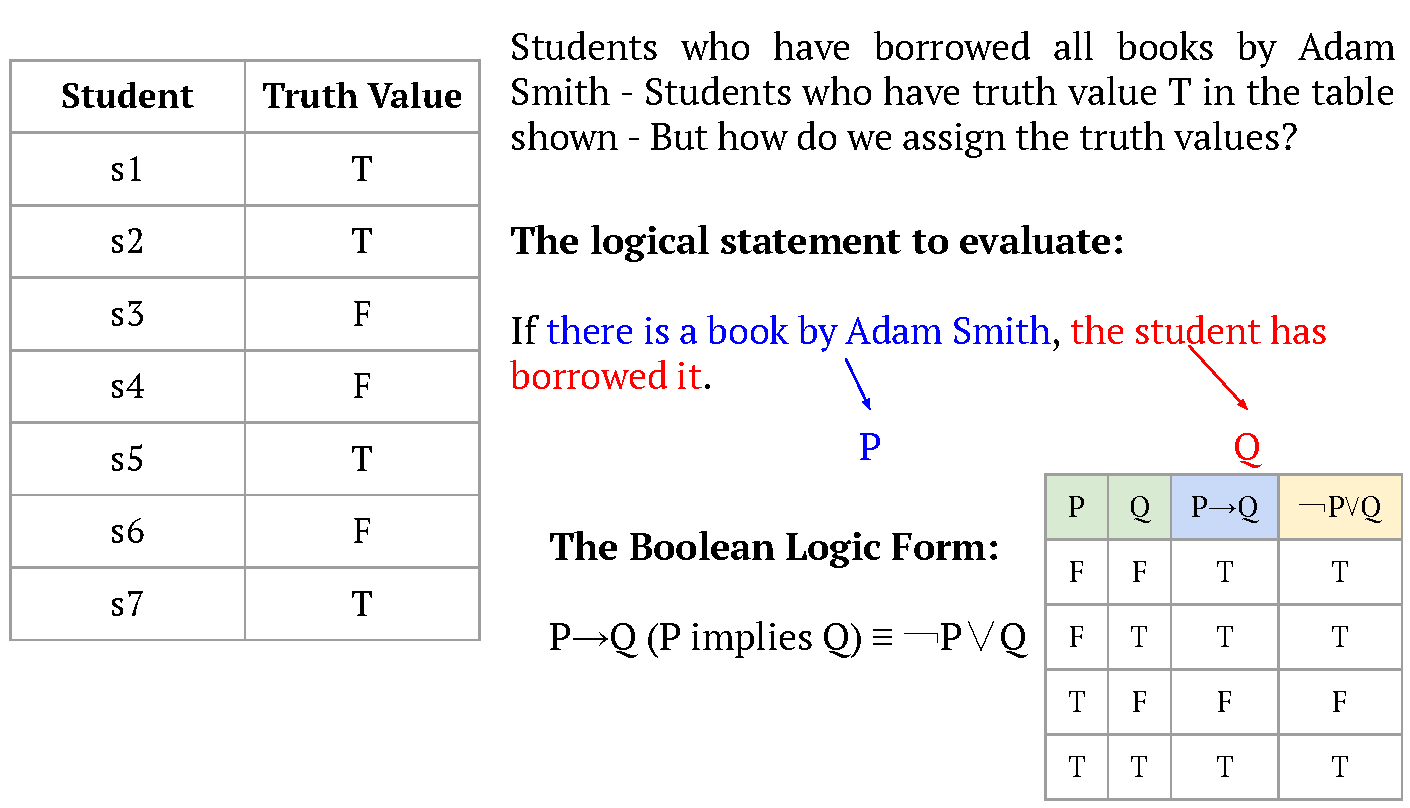
\includegraphics[scale=0.45]{tut_04_images/tut_04_02.pdf}
\end{center}
\end{frame}

\begin{frame}[fragile]{2(b). Borrowed \emph{All} of Adam Smith's Books}
\begin{center}
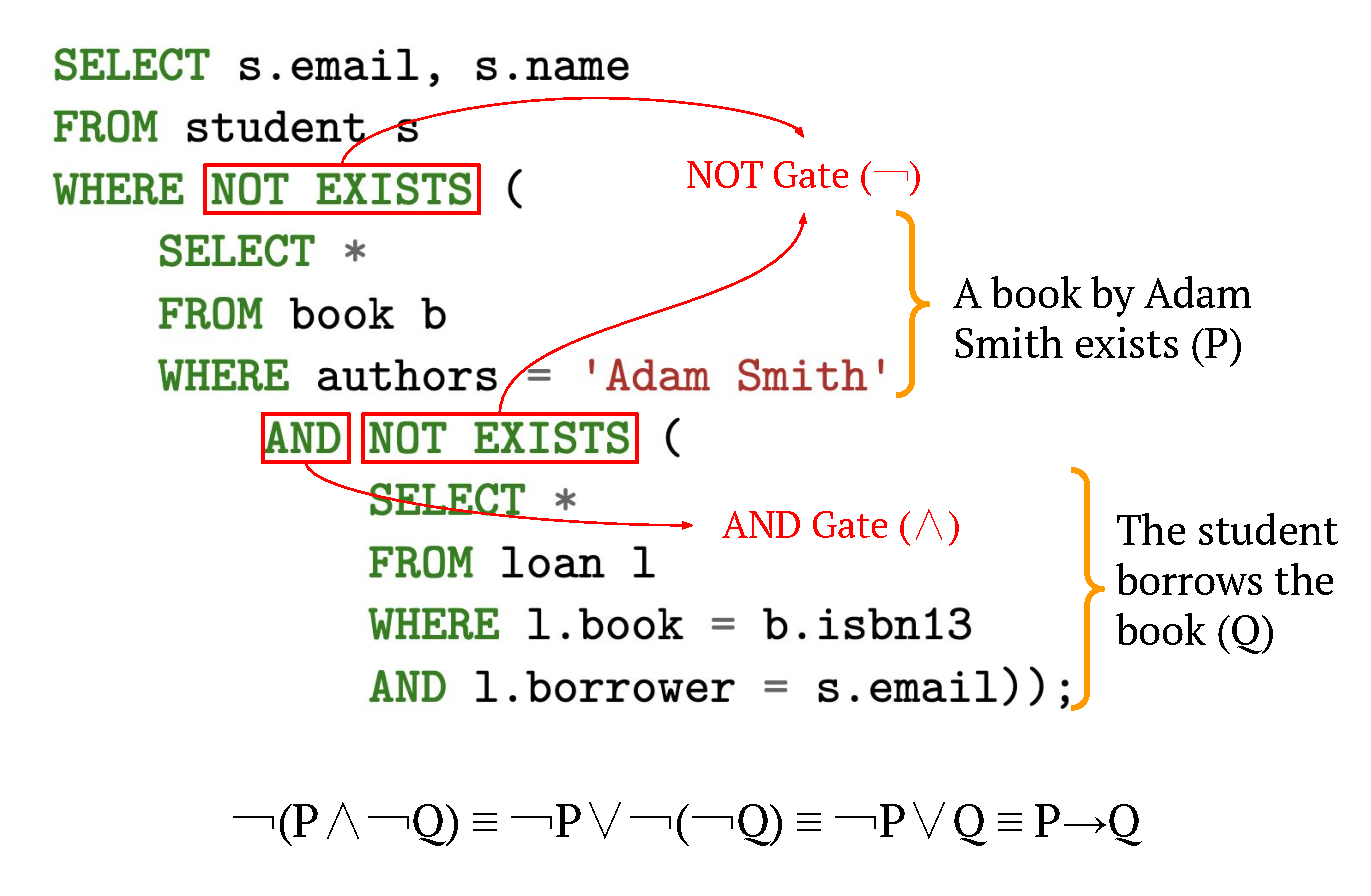
\includegraphics[scale=0.45]{tut_04_images/tut_04_01.pdf}
\end{center}
\end{frame}

\section{Discussion Queries}

\begin{frame}{Discussion: Aggregate, Nested \& Nested-Aggregate}
\small
\textit{To be discussed in class --- attempt before the tutorial; you may be called on to present.}
\begin{enumerate}
  \item[\textbf{3.}] \textbf{Aggregate Queries.} What are the average and the standard deviation of the duration of a loan, in days?
  \item[\textbf{4.}] \textbf{Nested Queries.} Print the names of the different students who own a copy of a book that they have \emph{never} lent to anybody.
  \item[\textbf{5.}] \textbf{Nested Aggregate Queries.} For each department, print the names of the students who lent the most.
\end{enumerate}
\end{frame}

\begin{frame}[fragile]{3. Average \& Standard Deviation of Loan Duration}
\small
A loan still out has no fixed duration yet --- same \texttt{COALESCE} trick as Tutorial 3's 1(c). \texttt{CEIL} rounds up to whole days.
\begin{lstlisting}[language=SQL]
SELECT CEIL(AVG(COALESCE(l.returned, CURRENT_DATE) - l.borrowed + 1)),
       CEIL(STDDEV_POP(COALESCE(l.returned, CURRENT_DATE)
                        - l.borrowed + 1))
FROM loan l;
\end{lstlisting}
\textbf{Keep it simple.} A nested-query alternative exists, but a single-table aggregate is the more natural fit here.
\end{frame}

\begin{frame}[fragile]{4. Owns a Copy, Never Lent It}
\small
\textbf{Inner query:} owners of a copy with no matching loan at all (i.e., that exact copy was never lent).
\begin{lstlisting}[language=SQL]
SELECT s.name
FROM student s
WHERE s.email IN (
  SELECT c.owner
  FROM copy c
  WHERE NOT EXISTS (
    SELECT * FROM loan l
    WHERE l.owner = c.owner AND l.book = c.book AND l.copy = c.copy
  )
);
\end{lstlisting}
We reduce the inner result to a \textbf{set of owners} first, \emph{then} look up names.
\end{frame}

\begin{frame}[fragile]{4. Why Not Just Join Student to Copy?}
\small
\begin{lstlisting}[language=SQL]
SELECT s.name
FROM student s, copy c
WHERE s.email = c.owner
  AND NOT EXISTS (
    SELECT * FROM loan l
    WHERE l.owner = c.owner AND l.book = c.book AND l.copy = c.copy
  );
\end{lstlisting}
\textbf{Incorrect.} A student with \emph{several} never-lent copies would have their name printed once per copy --- and we'd have no way to tell that apart from two different students who happen to share a name.
\end{frame}

\begin{frame}[fragile]{5. Who Lent the Most, per Department}
\small
Count each owner's loans, then keep only the rows whose count is \textbf{at least} every other same-department count.
\begin{lstlisting}[language=SQL]
SELECT s.department, s.name, COUNT(*)
FROM student s, loan l
WHERE l.owner = s.email
GROUP BY s.department, s.email, s.name
HAVING COUNT(*) >= ALL (
  SELECT COUNT(*)
  FROM student s1, loan l1
  WHERE l1.owner = s1.email
    AND s.department = s1.department
  GROUP BY s1.email
);
\end{lstlisting}
\textbf{Ties are real:} the Language department has \emph{multiple} top lenders --- exactly why one should avoid \texttt{TOP N} / \texttt{LIMIT} queries here.
\end{frame}

\begin{frame}{5. The Zero-Loan Edge Case}
\small
Suppose a new department, \emph{Undecidable Computations}, has students who have \textbf{never lent} a book.
\begin{itemize}
  \item Every one of them lent \textbf{0} books --- which is the maximum in that department.
  \item So they should \textbf{all} be printed, not none of them.
  \item But our query above never produces a $0$-count row for them at all: the \texttt{FROM student s, loan l} join silently \textbf{drops} students with no loans.
\end{itemize}
\textbf{Fix:} an \texttt{OUTER JOIN} from \texttt{student} to \texttt{loan}, with \texttt{CASE WHEN} / \texttt{ISNULL} to turn ``no matching loan'' into a count of $0$.
\medskip

\textbf{Also note:} we group by \texttt{s.name} purely to be able to \texttt{SELECT} it, even though \texttt{s.email} already determines it uniquely. PostgreSQL relaxes this rule --- but relying on that hurts portability.
\end{frame}

\section{Guidelines}

\begin{frame}{Guidelines \& Common Pitfalls}
\small
\begin{itemize}\itemsep4pt
  \item \textbf{Simple first.} If a single-table aggregate answers the question (Q3), prefer it over a nested rewrite.
  \item \textbf{Match the grain of the question.} ``Books never borrowed'' is about \texttt{book}, not \texttt{copy} --- don't join in a table that changes what ``never'' ranges over (2(a)).
  \item \textbf{Reduce, then look up.} For nested \texttt{IN}/\texttt{EXISTS} queries producing names, find the qualifying \emph{keys} first (in a subquery), then join for display columns --- joining too early can duplicate or misattribute rows (Q4).
  \item \textbf{Avoid \texttt{TOP N} / \texttt{LIMIT} for ``the most''.} Ties are common; \texttt{HAVING COUNT(*) >= ALL (\ldots)} naturally keeps every tied winner (Q5).
  \item \textbf{Mind the zero case.} A student/department with no matching rows can still be the correct answer --- \texttt{OUTER JOIN} + \texttt{CASE}/\texttt{ISNULL}, not an inner join, is what surfaces it (Q5).
\end{itemize}
\end{frame}

\begin{frame}
\begin{center}
Questions?\\
Drop a mail at: pratik.karmakar@u.nus.edu
\end{center}
\end{frame}

\end{document}
